\section{Evaluation}
\label{chapter:Evaluation}
We evaluated \textsc{TypeShield} by instrumenting various open source applications and analyzing the results. 
We used the two ftp server applications vsftpd (version 1.1.0) and proftpd (version 1.3.3), the two http server 
applications postgresql (version 9.0.10) and  mysql (5.1.65), the memory cache application memcached (version 1.4.20) 
and the node.js server application node (version 0.12.5). We chose these applications, which are a subset of the 
applications also used by the TypeAmor~\cite{veen:typearmor} to allow for later comparison.
In our evaluation we addressed the following research questions:
\begin{itemize}

 \item \textbf{RQ1:} How precise is \textsc{TypeShield} in recovering parameter count and type information for call-sites and call-targets from a given binary?

 \item \textbf{RQ2:} What level of security does \textsc{TypeShield} offer?
 We look at our implementation conceptually and assess qualitatievly whether our implementation can interfere with various classes of attacks. 
\todo[inline]{see the TypeAmor paper w.r.t. security analysis in the evaluation, a CDF figure is here required.}

% \item \textbf{RQ3:} What is the runtime performance overhead introduced by \textsc{TypeShield}?
% \todo[inline]{add a binary patch that does not crash none of the programs from SPEC2006.}
% \todo[inline]{need a table with all the results for each of the SPEC2006 programs and a bar diagram}
% 
% \item \textbf{RQ4:} What is the instrumentation overhead introduced by \textsc{TypeShield}?
% Here we measure how much the binaries increased in size after the instrumentation was added to the binaries.
%\todo[inline]{Measure the size (in bytes) of the SPEC2006 testes in RQ3 before and after adding all the patches}
\end{itemize}
\textbf{Comparison Method.} As we do not have access to the source code of TypeAmor, we implemented two modes in \textsc{TypeShield}. 
The first mode of our tool is an approximate implementation of the \textit{count} 
policy described by TypeArmor. The second mode is our implementation of the \textit{type} policy on
top of our \textit{count} policy implementation. 
%
%\textbf{Experimental Setup.} We setup our environment within a VirtualBox (version 5.0.26r) instance, which runs Kubuntu 16.04 LTS (Linux Kernel
%version 4.4.0) and has access to 3GB of RAM and 4 of 8 provided hardware threads (Intel i7-4170HQ @ 2.50 GHz).

\subsection{RQ1: Precision of \textsc{TypeShield}}
\label{section:typeshieldprecision}
\todo[inline]{In this section we need just one or two Table similar to what TypeArmor contains, first we need to define the fields which make most sense.}

To measure the precision of \textsc{TypeShield}, we need to compare the classification of call-sites and call-targets as is given by our tool to
some sort of ground truth for our test targets. We generate this ground truth by compiling our test targets using a custom compiled Clang/LLVM
compiler (version 4.0.0 trunk 283889) with a MachineFunction pass inside the x86 code generation implementation of LLVM. We essentially 
collect three data points for each call-site/call-target from our LLVM-pass:
\begin{itemize}
\item The point of origination, which is either the name of the call-target or the name of the function the call-site resides in.
\item The return type that is either expected by the call-site or provided by the call-target.
\item The parameter list that is provided by the call-site or expected by the call-target, which discards the variadic argument list.
\end{itemize}
However, before we can proceed to measure the quality and precision of \textsc{TypeShield}'s classification of call-targets and call-sites
using our ground truth, we need to evaluate the quality and applicability of the ground truth, we collected.

\subsubsection{Quality and Applicability of Ground Truth}
\label{subsection:typeshieldprecision}
To assess the applicability of our collected ground truth, we essentially need to assess the structural compatibility of our two datasets.
First, we take a look at the comparability of call-targets and second, we take a look at the compatibility of call-sites. The results are depcited in Table \ref{tbl:matchingquality}.

\begin{table}[h!]
\resizebox{\columnwidth}{!}{
	\begin{tabular}{l|r|r|r|r|r|r}%
	\toprule
	\multicolumn{1}{c}{\bfseries O2} & \multicolumn{3}{c|}{ {\bfseries call-targets}} & \multicolumn{3}{c}{{\bfseries call-sites} }\\
	\bfseries Target & match & Clang miss &  tool miss &  match & Clang miss & tool miss% specify table head
	\\\midrule
	\csvreader[before filter=\ifthenelse{\equal{\csvcoli}{geomean}}{\csvfilterreject}{\csvfilteraccept},  late after line=\\, late after last line=\\\midrule]{csvs/matching.O2.csv}{
		%1=\target, 2=\opt, 3=\fns, 4=\fnsnotClang, 5=\fnsnotpadyn, 6=\ats, 7=\atnotClang, 8=\atnotpadyn, 9=\cscount, 10=\csClang, 11=\cspadyn
	}
	{\csvcoli & \csvcoliii & \csvcoliv (\csvcolv \% )& \csvcolvi (\csvcolvii \% )& \csvcolxiii & \csvcolxiv  (\csvcolxv) & \csvcolxvi   (\csvcolvii) }% specify your coloumns here

	\csvreader[before filter=\ifthenelse{\equal{\csvcoli}{geomean}}{\csvfilteraccept}{\csvfilterreject},  late after line=\\, late after last line=\\\bottomrule]{csvs/matching.O2.csv}{
		%1=\target, 2=\opt, 3=\fns, 4=\fnsnotClang, 5=\fnsnotpadyn, 6=\ats, 7=\atnotClang, 8=\atnotpadyn, 9=\cscount, 10=\csClang, 11=\cspadyn
	}
	{\csvcoli & \csvcoliii & \csvcoliv (\csvcolv \% )& \csvcolvi (\csvcolvii \% )& \csvcolxiii & \csvcolxiv  (\csvcolxv) & \csvcolxvi   (\csvcolvii) }% specify your coloumns here
    	\end{tabular}}
%     	}
	\caption {Table shows the quality of structural matching provided by our automated verify and test environment, 
	regarding call-sites and call-targets when compiling with optimization level O2. The label Clang miss 
	denotes elements not found in the data-set of the Clang/LLVM pass. The label tool miss denotes elements not found in the data-set of \textsc{TypeShield}.}
	\label{tbl:matchingquality}
\end{table}

\textbf{Call-targets.} The obvious choice for structural comparison regarding call-targets is their name, as these are simply functions. 
First, we have to remove internal functions from our data-sets like the \texttt{\_init} or \texttt{\_fini} functions, which are of no consequence for us. 
Furthermore, while C functions can simply be matched by their name as they are unique through the binary, the same cannot be said about the 
language C++. One of the key differences between C and C++ is function overloading, which allows to define several functions with the same name, as 
long as they differ in namespace or parameter type. As LLVM does not know about either concept, the Clang compiler needs to generate unique names. 
The method used for unique name generation is called mangling and composes the actual name of the function, its the return type, its name-space and the 
types of its parameter list. We therefore need to reverse this process and then compare the fully typed names.
Table \ref{tbl:matchingquality} shows three data points regarding call-targets for the optimization level O2:
\begin{itemize}
\item The number of comparable call-targets that are found in both datasets
\item Clang miss: The number of call-targets that are found by \textsc{TypeShield} but not by our Clang/LLVM pass
\item tool miss: The number of call-targets that are found by our Clang/LLVM pass but not by \textsc{TypeShield}
\end{itemize}
The problematic column is the Clang miss column, as these might indicate problems with \textsc{TypeShield}. These numbers are relatively low (below 1\%) with only node showing a significant higher value than the rest (around 1.6\%). The column labeled tool miss lists 
higher numbers, however these are of no real concern to us, as our ground truth pass possibly collects more data: All source files used during the 
compilation of our test-targets are incorporated into our ground truth. The compilation might generate more than one binary and therefore not 
necessary all source files are used for our test-target.

Considering this, we can safely state that our structural matching between ground truth and \textsc{TypeShield} regarding call-targets is nearly
perfect (above 98\%)\\


\textbf{Call-sites.} While our structural matching of call-targets is rather simple, the matter of matching callsites is more complex. Our tool can provide accurate addressing of call-sites within the binary. However, Clang/LLVM does not have such capabilities in its intermediate representation (IR). Furthermore the IR is not the final representation within the compiler, as the IR is transformed into a machine-based representation (MR), which is the again optimized. Although we can read information regarding paramters from the IR, it is not possible with the MR. Therefore we attach that data directly after the conversion from IR to MR and read that data at the end of the compilation. To not unneccessarily pollute our dataset, we only considered call-targets, which have been found in both datasets. 
The table \ref{tbl:matchingquality} shows three data points regarding call-sites for the optimization level O2:
\begin{itemize}
\item The number of comparable call-sites that are found in both datasets.
\item Clang miss: The number of call-sites that are discarded from the dataset of \textsc{TypeShield}.
\item tool miss: The number of call-sites that are discarded from the dataset of our Clang/LLVM pass.
\end{itemize}

Both columns (Clang miss and tool miss) show a relatively low number of problems (<0.5\%), therefore we can also safely state that our structural matching between ground truth and \textsc{TypeShield} regarding call-sites is also nearly perfect (above 99\%)

\subsubsection{Classification Precision (\textit{count})}
\label{subsection:typeshieldcountprecision}

We measured two data points per target, the number and ratio of perfect classifications and the number and ratio of problematic classifications, which in the case of calltargets refers to overestimations and in case of callsites refers to underestimations. The results are depicted in Table \ref{tbl:precisionCOUNT}.
\begin{table}[h!]
\resizebox{\columnwidth}{!}{
	\begin{tabular}{l|r|r|r|r|r|r}%

	\toprule
	\multicolumn{1}{c}{\bfseries O2} & \multicolumn{3}{c}{\bfseries Call-targets} & \multicolumn{3}{c}{\bfseries Call-sites}\\
	
	\bfseries Target & \#  &  perfect &  problem & \# & perfect &  problem % specify table head
	\\\midrule
	\csvreader[before filter=\ifthenelse{\equal{\csvcolii}{geomean}}{\csvfilterreject}{\csvfilteraccept}, late after line=\\, late after last line=\\\midrule]{csvs/classification_comp.sources_union_follow.O2.csv}{
		%1=opt,2=target,3=cs,4=cs args,5=perfect,6=cs args,7=problem,8 = cs non-void ,9=correct,10 = cs non-void, 11=problem,12 = ct, 13 = ct args, 14=perfect, 15 = ct args, 16=problem, 17 = ct void, 18=correct, 19=ct void, 20=problem
}
	{\csvcolii  &  \csvcolxii & \csvcolxiii \ (\csvcolxiv \%) & \csvcolxv \ (\csvcolxvi \%) & \csvcoliii & \csvcoliv \ (\csvcolv \%) & \csvcolvi \ (\csvcolvii\%)}% specify your coloumns here

	\csvreader[before filter=\ifthenelse{\equal{\csvcolii}{geomean}}{\csvfilteraccept}{\csvfilterreject}, late after line=\\, late after last line=\\\bottomrule]{csvs/classification_comp.sources_union_follow.O2.csv}{
		%1=opt,2=target,3=cs,4=cs args,5=perfect,6=cs args,7=problem,8 = cs non-void ,9=correct,10 = cs non-void, 11=problem,12 = ct, 13 = ct args, 14=perfect, 15 = ct args, 16=problem, 17 = ct void, 18=correct, 19=ct void, 20=problem
}
	{\csvcolii  &  \csvcolxii & \csvcolxiii \ (\csvcolxiv \%) & \csvcolxv \ (\csvcolxvi \%) & \csvcoliii & \csvcoliv \ (\csvcolv \%) & \csvcolvi \ (\csvcolvii\%)}% specify your coloumns here
    	\end{tabular}

}
		\caption {The results for analysis using the \textit{count} policy on the O2 optimization level.}
		\label{tbl:precisionCOUNT}
\end{table}~\\
\textbf{Experiment Setup (Call-targets)}
{Union combination operator with an $analyze$ function that follows into occurring direct calls.
}\\~\\
\textbf{Results (Call-targets)}{
The problem rate is under 0.01\%, as there are only two testtargets, that exhibit a problematic classification. The rate of perfect classification is in general over 80\% with mysql as an exception (73.85\%) resulting in a geometric mean of 86.86\%.
}\\~\\
\textbf{Experiment Setup (Call-sites)}
{ Union combination operator with an $analyze$ function that does not follow into occurring direct calls while relying on a backward inter-procedural analysis.
}\\~\\
\textbf{Results (Call-sites)} {
The problem rate is under 0.01\%, as there is only one testtarget, that exhibit a problematic classification. The rate of perfect classification is in general over 60\% with nginx (48.49\%) and node (56.34\%) as an exception resulting in a geometric mean of 71.97\%.}


\subsubsection{Classification Precision (\textit{type})}
\label{subsection:typeshieldcountprecision}

We measured two data points per testtarget, the number and ratio of perfect classifications and the number and ratio of problematic classifications, which in the case of calltargets refers to overestimations and in case of callsites refers to underestimations. The results are depicted in Table \ref{tbl:precisionTYPE}.
\begin{table}[h!]
\resizebox{\columnwidth}{!}{
	\begin{tabular}{l|r|r|r|r|r|r}%

	\toprule
	\multicolumn{1}{c}{\bfseries O2} & \multicolumn{3}{c}{\bfseries Call-targets} & \multicolumn{3}{c}{\bfseries Call-sites}\\
	
	\bfseries Target & \#  &  perfect &  problem & \# & perfect &  problem % specify table head
	\\\midrule
	\csvreader[before filter=\ifthenelse{\equal{\csvcolii}{geomean}}{\csvfilterreject}{\csvfilteraccept},  late after line=\\, late after last line=\\\midrule]{csvs/classification_comp2.type_exp6.O2.csv}{
		%1=opt,2=target,3=cs,4=cs args,5=perfect,6=cs args,7=problem,8 = cs non-void ,9=correct,10 = cs non-void, 11=problem,12 = ct, 13 = ct args, 14=perfect, 15 = ct args, 16=problem, 17 = ct void, 18=correct, 19=ct void, 20=problem
}
	{\csvcolii  &  \csvcolxii & \csvcolxiii \ (\csvcolxiv \%) & \csvcolxv \ (\csvcolxvi \%) & \csvcoliii & \csvcoliv \ (\csvcolv \%) & \csvcolvi \ (\csvcolvii\%)}% specify your coloumns here

	\csvreader[before filter=\ifthenelse{\equal{\csvcolii}{geomean}}{\csvfilteraccept}{\csvfilterreject},  late after line=\\, late after last line=\\\bottomrule]{csvs/classification_comp2.type_exp6.O2.csv}{
		%1=opt,2=target,3=cs,4=cs args,5=perfect,6=cs args,7=problem,8 = cs non-void ,9=correct,10 = cs non-void, 11=problem,12 = ct, 13 = ct args, 14=perfect, 15 = ct args, 16=problem, 17 = ct void, 18=correct, 19=ct void, 20=problem
}
	{\csvcolii  &  \csvcolxii & \csvcolxiii \ (\csvcolxiv \%) & \csvcolxv \ (\csvcolxvi \%) & \csvcoliii & \csvcoliv \ (\csvcolv \%) & \csvcolvi \ (\csvcolvii\%)}% specify your coloumns here
    	\end{tabular}

}
		\caption {The results for analysis using the \textit{type} policy on the O2 optimization level.}
		\label{tbl:precisionTYPE}
\end{table}~\\
\textbf{Experiment Setup (Call-targets)}
{Union combination operator with an $analyze$ function that does follow into occurring direct calls  and a vertical merge that intersects all reads until the first write.
}\\~\\
\textbf{Results (Call-targets)}{
For half of the set, the problem rate is under 1\% and for the other half it is not above 10\%, resulting in a geomean of 1.92\%. The rate of perfect classification is in general over 70\% with nginx (69.38\%) and mysql (63.16\%)  resulting in a geometric mean of 77.15\%.
}\\~\\
\textbf{Experiment Setup (Call-sites)}
{ Union combination operator with an $analyze$ function that does not follow into occurring direct calls while relying on a backward inter-procedural analysis.
}\\~\\
\textbf{Results (Call-sites)} {
For two thirds of the set, the problem rate is under 2\% and for last third it is not above 10\%, resulting in a geomean of 1.38\%.  The rate of perfect classification is in general over 50\% with node (44.76\%) as an exception resulting in a geometric mean of 68.35\%.}


%
%
%Efficiency
%
%
\subsection{RQ2: Security Level of \textsc{TypeShield}}
\label{section:typeshieldeffectiveness}
\todo[inline]{In this section we need just one or two Table similar to what TypeArmor contains, 
first we need to define the fields which make most sense.}

%\begin{figure}[htbp!]
%  \centering
%  \resizebox{1.04\columnwidth}{!}{\includesvg{postgresqlO2}}
%  \caption{svg image}
%\end{figure}

\begin{table*}[htbp!]
\begin{center}
 \resizebox{2\columnwidth}{!}{
	\begin{tabular}{l|r|rcl|r|rcl|r|rcl|r|rcl|r}%

	\toprule
	\multicolumn{1}{c}{\bfseries O2} & \multicolumn{1}{c}{\bfseries AT} & \multicolumn{4}{c}{\bfseries \textit{count}*} & \multicolumn{4}{c}{\bfseries \textit{count}} & \multicolumn{4}{c}{\bfseries \textit{type}*} & \multicolumn{4}{c}{\bfseries \textit{type}}\\
	
	\bfseries Target && \multicolumn{3}{c}{ limit (mean $\pm$ $\sigma$)} & median & \multicolumn{3}{c}{ limit (mean $\pm$ $\sigma$)} & median & \multicolumn{3}{c}{ limit (mean $\pm$ $\sigma$)} & median & \multicolumn{3}{c}{ limit (mean $\pm$ $\sigma$)} & median  % specify table head
	\\\midrule
	\csvreader[before filter=\ifthenelse{\equal{\csvcolii}{geomean}}{\csvfilterreject}{\csvfilteraccept},  late after line=\\, late after last line=\\\midrule]{csvs/policy_compare_at.O2.csv}{
	%1=opt,2=target,3=at,4=count safe avg,5=count safe sig,6=count safe median,7=count prec avg,8=count prec sig,9=count prec median,10=count* avg,11=count* sig,12=count* median,13=type safe avg,14=type safe sig,15=type safe median,16=type prec avg,17=type prec sig,18=type prec median,19=type* avg,20=type* sig,21=type* median
 }
	{\csvcolii  &  \csvcoliii & \csvcolx & $\pm$ & \csvcolxi & \csvcolxii & \csvcolvii & $\pm$ & \csvcolviii& \csvcolix& \csvcolxix & $\pm$ & \csvcolxx& \csvcolxxi & \csvcolxvi & $\pm$ & \csvcolxvii& \csvcolxviii }% specify your coloumns here

	\csvreader[before filter=\ifthenelse{\equal{\csvcolii}{geomean}}{\csvfilteraccept}{\csvfilterreject},  late after line=\\, late after last line=\\\bottomrule]{csvs/policy_compare_at.O2.csv}{
	%1=opt,2=target,3=at,4=count safe avg,5=count safe sig,6=count safe median,7=count prec avg,8=count prec sig,9=count prec median,10=count* avg,11=count* sig,12=count* median,13=type safe avg,14=type safe sig,15=type safe median,16=type prec avg,17=type prec sig,18=type prec median,19=type* avg,20=type* sig,21=type* median
 }
	{\csvcolii  &  \csvcoliii & \csvcolx & $\pm$ & \csvcolxi & \csvcolxii & \csvcolvii & $\pm$ & \csvcolviii& \csvcolix& \csvcolxix & $\pm$ & \csvcolxx& \csvcolxxi & \csvcolxvi & $\pm$ & \csvcolxvii& \csvcolxviii }% specify your coloumns here

    	\end{tabular}

}
	\caption {The results of comparing our implementation results with the theoretical limits for the different restriction policies combined with an address taken analysis for optimization level O2.}
	\label{tbl:policycompat}
\end{center}
\end{table*}

We are now going to evaluate the effectiveness of \textsc{TypeShield} leveraging the result of several experiment runs: First we are going to establish a baseline using the data 
collected from our Clang/LLVM pass, which are the theoretical limits our implementation can reach for both the \textit{count} and the \textit{type} schema. Second we are going to evaluate the effectiveness of our \textit{count} 
policy and third we are going to evaluate the effectiveness of our \textit{type} policy. For each series we collected three data points per test target, the average number of call-targets per call-site, the standard deviation $\sigma$ and the median. The results are depicted in table \ref{tbl:policycompat}. 

\subsubsection{Theoretical Limits.}
\label{subsection:theoreticallimit}
We explore the theoretical limits regarding the effectiveness of the \textit{count} and \textit{type} policies by relying on the collected ground truth data, essentially assuming perfect classification.

~\\
\textbf{Experiment Setup} Based on the type information collected by our Clang/LLVM pass, we conducted two experiment series.
We derived the available number of call-targets for each call-site based on the collected ground truth applying the \textit{count} and \textit{type} schema


~\\
\textbf{Results:}
\begin{itemize}
\item The theoretical limit of the \textit{count*} schema has a geometric mean of 233 possible call-targets, which is 16.48\% of the geometric mean of total available 
call-targets.
\item The theoretical limit of the \textit{type*} schema has a geometric mean of 210 possible call-targets, which is 14.86\% of the geometric mean of total available
call-targets.
\end{itemize}

When compared, the theoretical limit of the \textit{type} policy allows about 10\% less available call-targets in the geomean in O2 than the limit of the \textit{count} policy.

\subsubsection{\textsc{TypeShield} implementation}
\label{subsection:typeshieldvslimitcount}

\textbf{Experiment Setup.} We setup our two experiment series based on our previous evaluations regarding the classification precision for the \textit{count} and the \textit{type} policy.

~\\
\textbf{Results.}
\begin{itemize}
\item The \textit{count} schema has a geometric mean of 315 possible call-targets, which is 22.29\% of the geometric mean of total available 
call-targets. This is 35.19\% more than the theoretical limit of available call-targets per call-site.
\item The \textit{type} schema has a geometric mean of 290 possible call-targets, which is 20.52\% of the geometric mean of total available
call-targets. This is 38.09\% more than the theoretical limit of available call-targets per call-site.
\end{itemize}

When compared, our implementation of the \textit{type} policy allows about 7.93\% less available call-targets in the geomean in O2 than our implementation of the \textit{type} policy.


%\begin{table}[h!]
%\resizebox{.4\textwidth}{!}{
%	\begin{tabular}{l|c|rcl|c|rcl|c}%
%
%	\toprule
%	\multicolumn{1}{c}{\bfseries O2} & \multicolumn{1}{c}{\bfseries AT} & \multicolumn{4}{c}{\bfseries \textit{count} safe} & \multicolumn{4}{c}{\bfseries \textit{count} prec}\\
%	
%	\bfseries Target && \multicolumn{3}{c}{ limit (mean $\pm$ $\sigma$)} & median & \multicolumn{3}{c}{ limit (mean $\pm$ $\sigma$)} & median  % specify table head
%	\\\midrule
%	\csvreader[ late after line=\\, late after last line=\\\midrule]{../MA_Pictures/policy_compare_at.O2.csv}{
%	%1=opt,2=target,3=at,4=count safe avg,5=count safe sig,6=count safe median,7=count prec avg,8=count prec sig,9=count prec median,10=count* avg,11=count* sig,12=count* median,13=type safe avg,14=type safe sig,15=type safe median,16=type prec avg,17=type prec sig,18=type prec median,19=type* avg,20=type* sig,21=type* median
% }
%	{\csvcolii  &  \csvcoliii & \csvcoliv & $\pm$ & \csvcolv & \csvcolvi & \csvcolvii & $\pm$ & \csvcolviii& \csvcolix}% specify your coloumns here
%
%    	\end{tabular}
%}
%		\caption {The results of comparing \textit{count} safe and precision implementation restricted using an address taken analysis throughout different optimizations.}
%		\label{tbl:policycompatcount}
%\end{table}
%
%\begin{table}[h!]
%\resizebox{.4\textwidth}{!}{
%	\begin{tabular}{l|c|rcl|c|rcl|c}%
%
%	\toprule
%	\multicolumn{1}{c}{\bfseries O2} & \multicolumn{1}{c}{\bfseries AT} & \multicolumn{4}{c}{\bfseries \textit{type} safe} & \multicolumn{4}{c}{\bfseries \textit{type} prec}\\
%	
%	\bfseries Target && \multicolumn{3}{c}{ limit (mean $\pm$ $\sigma$)} & median & \multicolumn{3}{c}{ limit (mean $\pm$ $\sigma$)} & median  % specify table head
%	\\\midrule
%	\csvreader[ late after line=\\, late after last line=\\\midrule]{../MA_Pictures/policy_compare_at.O2.csv}{
%	%1=opt,2=target,3=at,4=count safe avg,5=count safe sig,6=count safe median,7=count prec avg,8=count prec sig,9=count prec median,10=count* avg,11=count* sig,12=count* median,13=type safe avg,14=type safe sig,15=type safe median,16=type prec avg,17=type prec sig,18=type prec median,19=type* avg,20=type* sig,21=type* median
% }
%	{\csvcolii  &  \csvcoliii & \csvcolxiii & $\pm$ & \csvcolxiv & \csvcolxv & \csvcolxvi & $\pm$ & \csvcolxvii& \csvcolxviii}% specify your coloumns here
%
%    	\end{tabular}
%}
%		\caption {The results of comparing \textit{type} safe and precision implementation restricted using an address taken analysis throughout different optimizations.}
%		\label{tbl:policycompattype}
%\end{table}

%
%\newpage
%\section{Security Analysis of \textsc{TypeShield}}
%\label{section:typeshieldsecurityanalysis}
%
%In this section, we discuss how effective \textsc{TypeShield} is 
%stopping advance code-reuse attacks (CRAs).
%Patching Policies
%Two types of diagrams. Table 5 from TypeArmor and a CDF to compare param count and param type. (baseline)
%here we put the CDF graphs from. There is no accurate security metrics to asses the security level of the enforced policy.
%
%
%
%\begin{table}
%\centering
%\resizebox{0.8\textwidth}{!}{
%	\begin{tabular}{l|c|c|c|c|c|c|c|c|c}%
%	\toprule
%	\multicolumn{1}{c}{\bfseries O0} & \multicolumn{1}{c}{} & \multicolumn{8}{|c}{ {\bfseries parameters}} \\
%	\bfseries Target & \bfseries \#CS & \bfseries -x & \bfseries +0 & \bfseries +1 & \bfseries +2 & \bfseries +3 & \bfseries +4 & \bfseries +5 & \bfseries +6 % specify table head
%	\\\midrule
%	\csvreader[ late after line=\\, late after last line=\\\midrule]{../MA_Pictures/classification_cs.O0.csv}{
%		%1=target,2=opt,3=cs,4=problems,5=+0,6=+1,7=+2,8=+3,9=+4,10=+5,11=+6,12=non-void-ok,13=non-void-problem
%	}
%	{\csvcoli & \csvcoliii & \csvcoliv & \csvcolv & \csvcolvi & \csvcolvii & \csvcolviii & \csvcolix & \csvcolx & \csvcolxi }% specify your coloumns here
%
%	\multicolumn{1}{c}{\bfseries O1}
%	\\\midrule
%	\csvreader[ late after line=\\, late after last line=\\\midrule]{../MA_Pictures/classification_cs.O1.csv}{
%		%1=target,2=opt,3=cs,4=problems,5=+0,6=+1,7=+2,8=+3,9=+4,10=+5,11=+6,12=non-void-ok,13=non-void-problem
%	}
%	{\csvcoli & \csvcoliii & \csvcoliv & \csvcolv & \csvcolvi & \csvcolvii & \csvcolviii & \csvcolix & \csvcolx & \csvcolxi}% specify your coloumns here
%
%	\multicolumn{1}{c}{\bfseries O2}
%	\\\midrule
%	\csvreader[ late after line=\\, late after last line=\\\midrule]{../MA_Pictures/classification_cs.O2.csv}{
%		%1=target,2=opt,3=cs,4=problems,5=+0,6=+1,7=+2,8=+3,9=+4,10=+5,11=+6,12=non-void-ok,13=non-void-problem
%	}
%	{\csvcoli & \csvcoliii & \csvcoliv & \csvcolv & \csvcolvi & \csvcolvii & \csvcolviii & \csvcolix & \csvcolx & \csvcolxi}% specify your coloumns here
%
%	\multicolumn{1}{c}{\bfseries O3}
%	\\\midrule
%	\csvreader[ late after line=\\, late after last line=\\\bottomrule]{../MA_Pictures/classification_cs.O3.csv}{
%		%1=target,2=opt,3=cs,4=problems,5=+0,6=+1,7=+2,8=+3,9=+4,10=+5,11=+6,12=non-void-ok,13=non-void-problem
%	}
%	{\csvcoli & \csvcoliii & \csvcoliv & \csvcolv & \csvcolvi & \csvcolvii & \csvcolviii & \csvcolix & \csvcolx & \csvcolxi}% specify your coloumns here
%
%
%    	\end{tabular}
%	}
%		\caption {Table shows the overestimation of the parameter count in matched callsites occurring in our precision focussed implementation of the \textit{count} policy, with -x denoting problematic callsites, when compiling with optimization levels O0 through O3}
%	\label{tbl:baselinecs}
%\end{table}
%
%\begin{figure}
%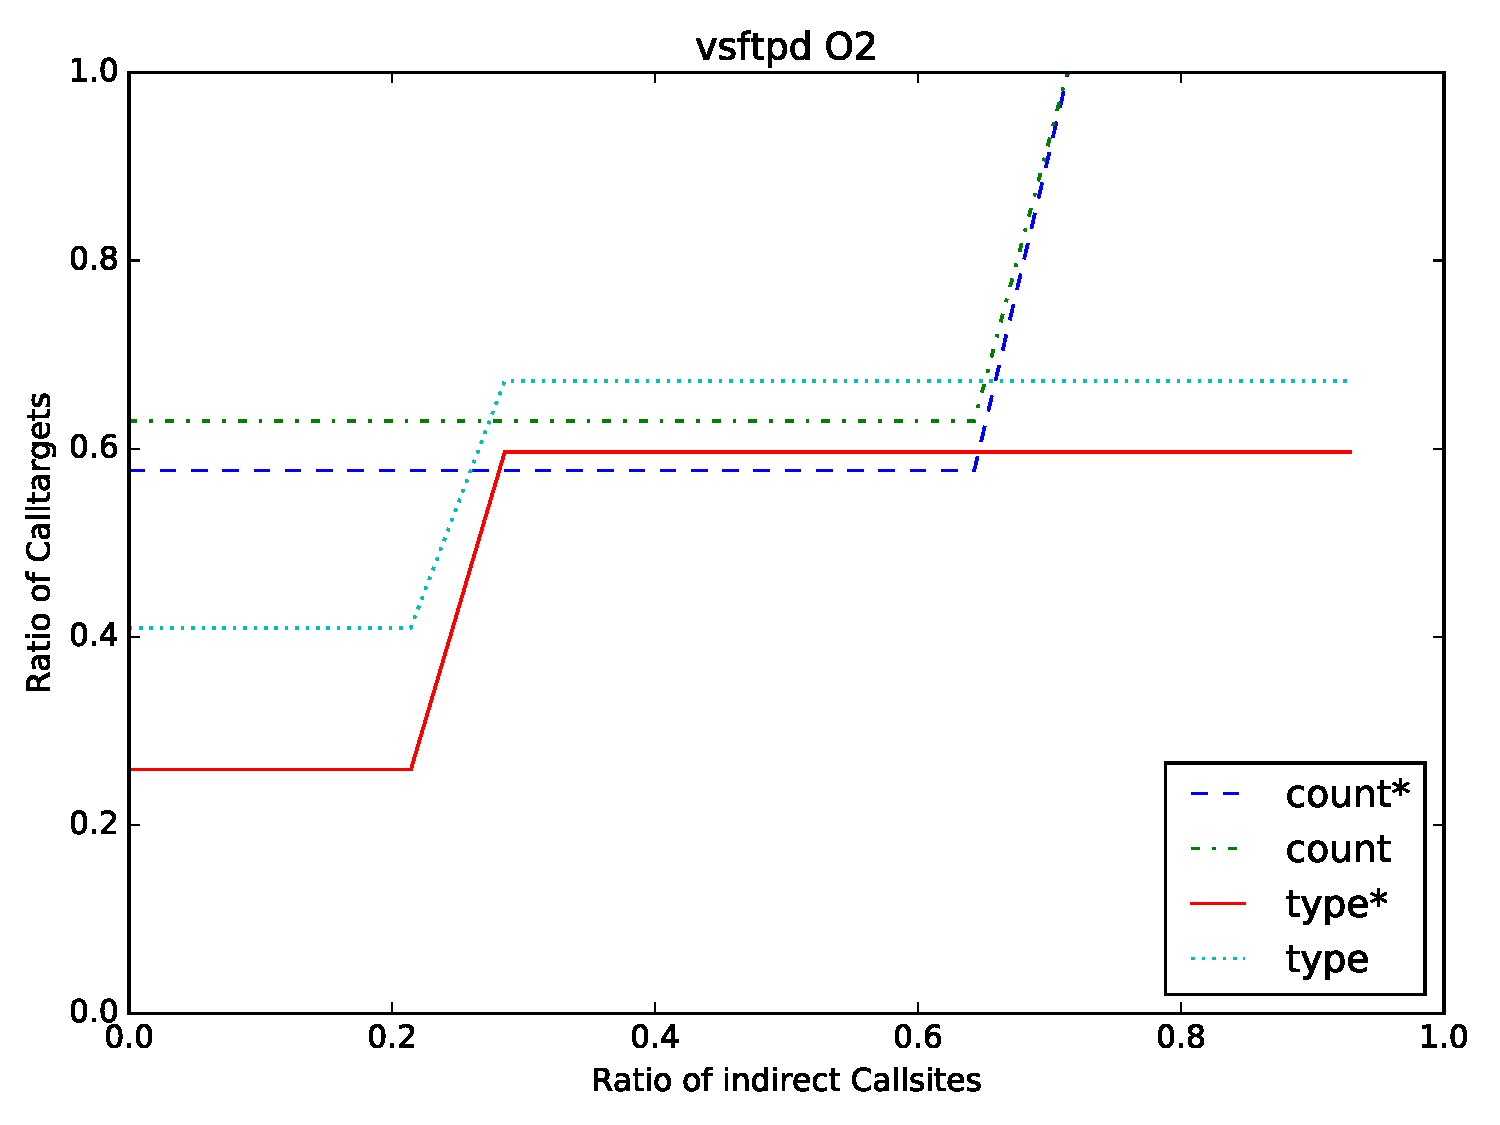
\includegraphics[width=0.5\textwidth]{../MA_Pictures/vsftpd.pdf}
%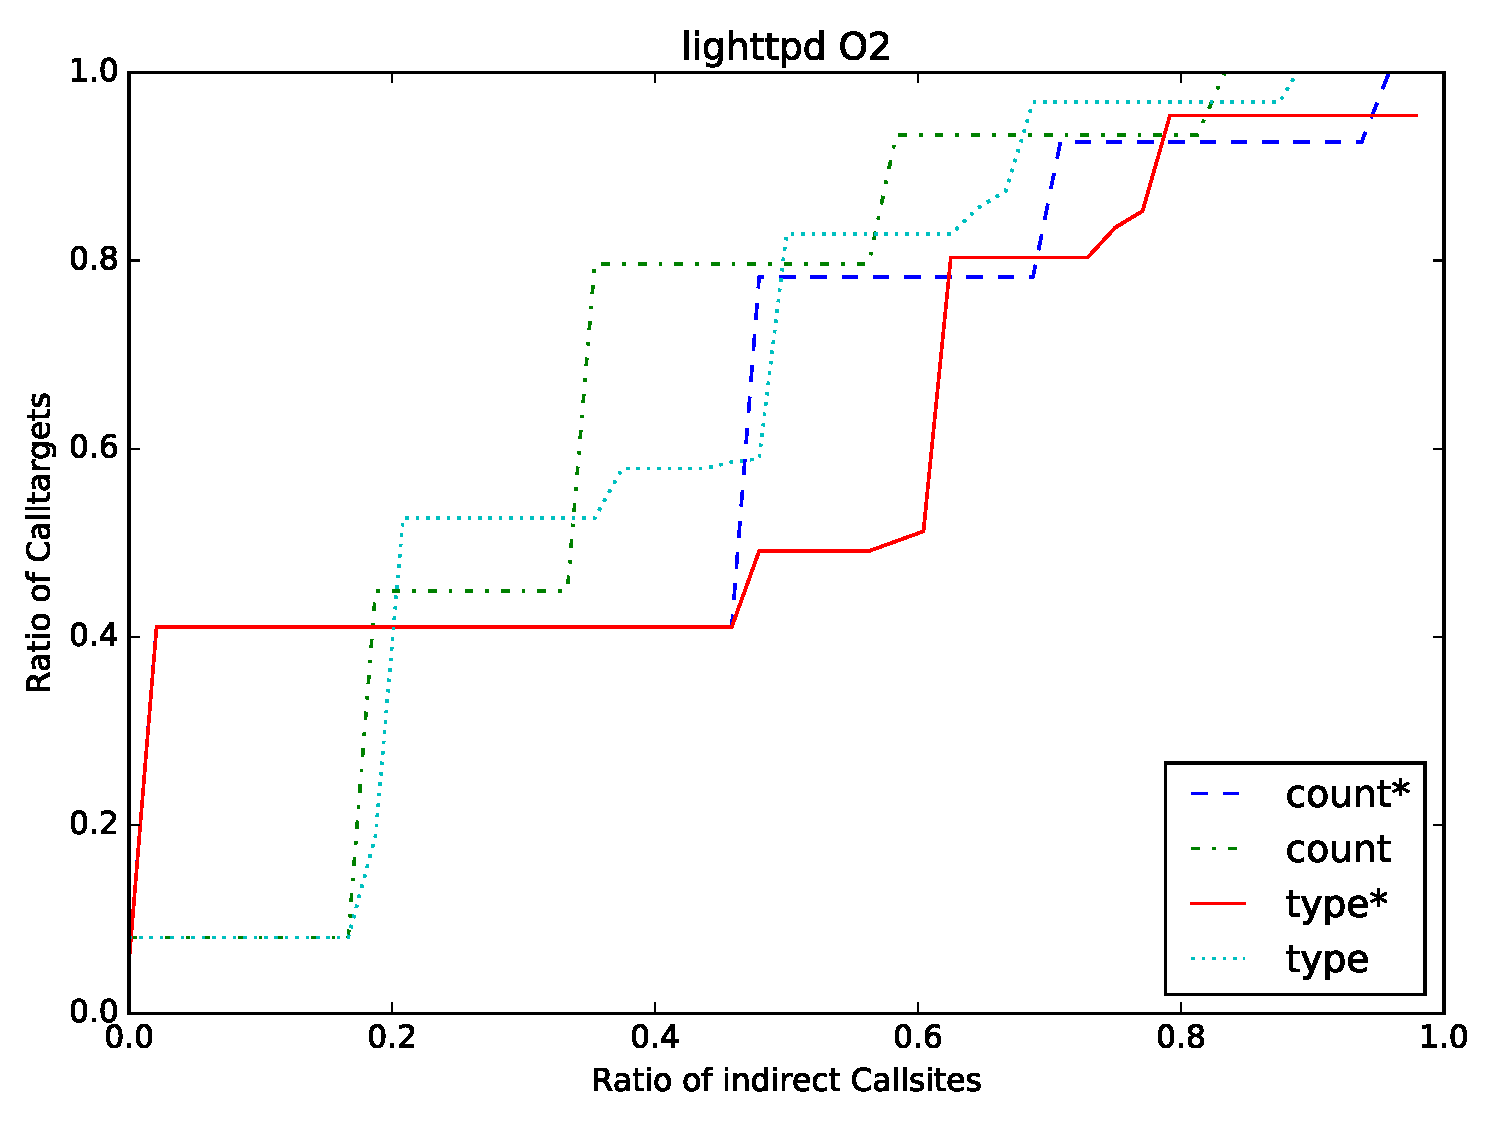
\includegraphics[width=0.5\textwidth]{../MA_Pictures/lighttpd.pdf}\\
%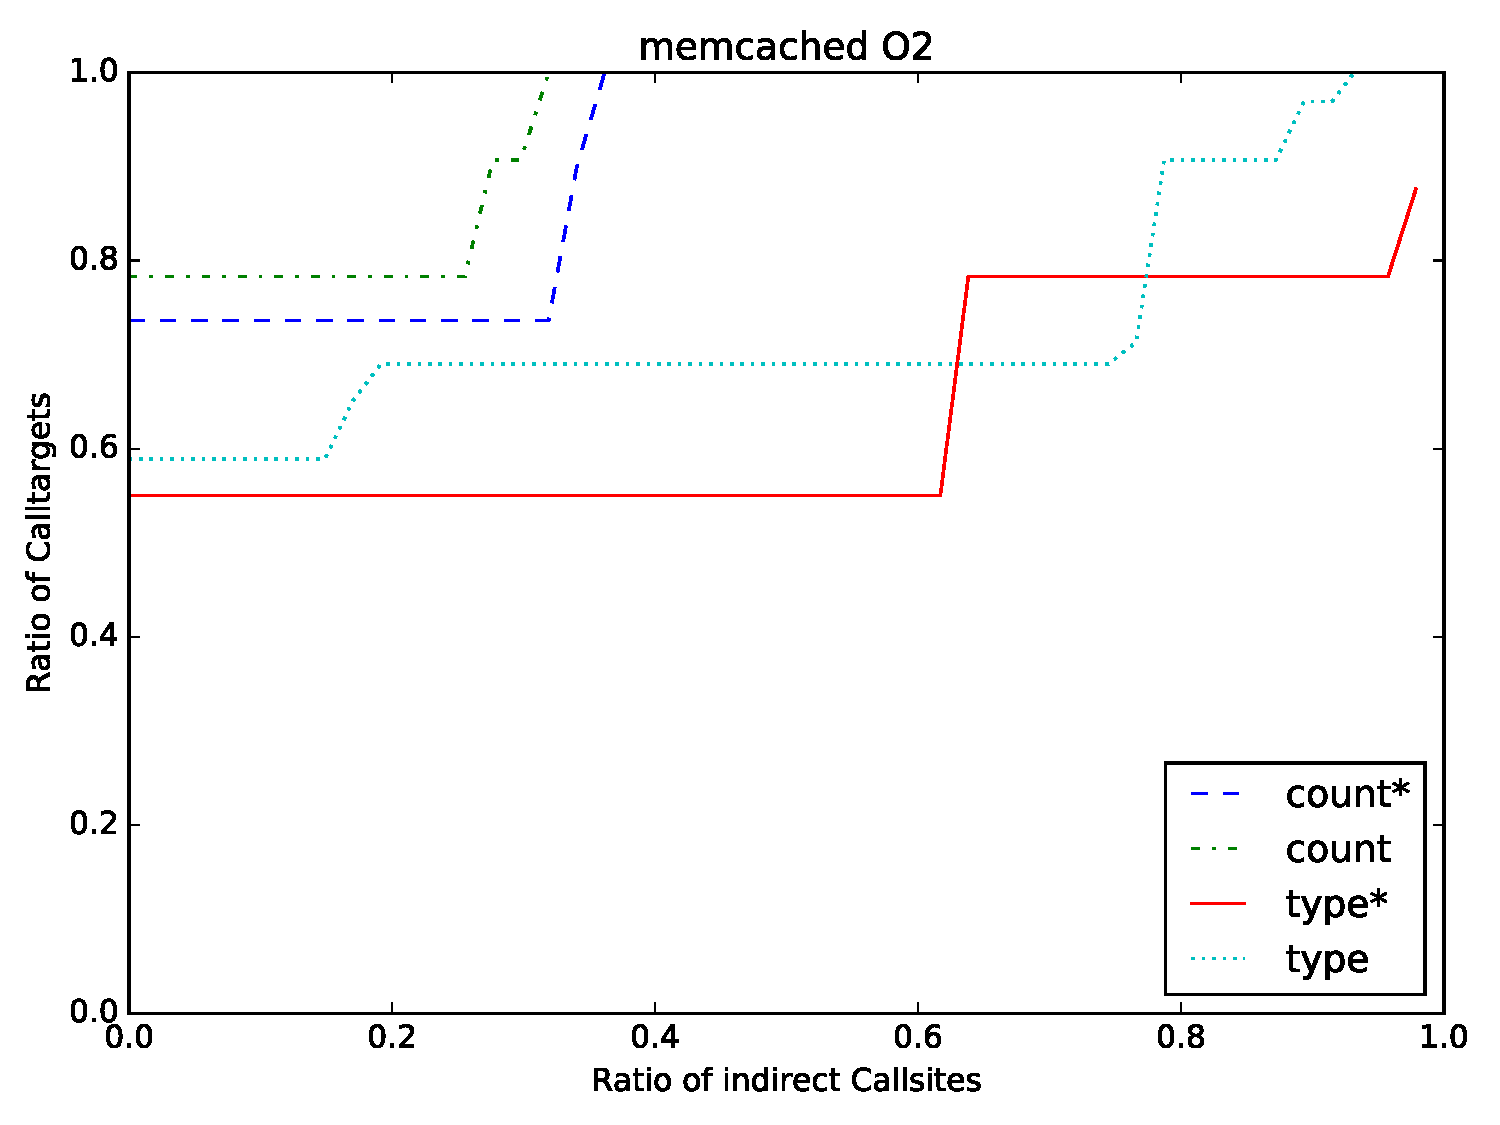
\includegraphics[width=0.5\textwidth]{../MA_Pictures/memcached.pdf}
%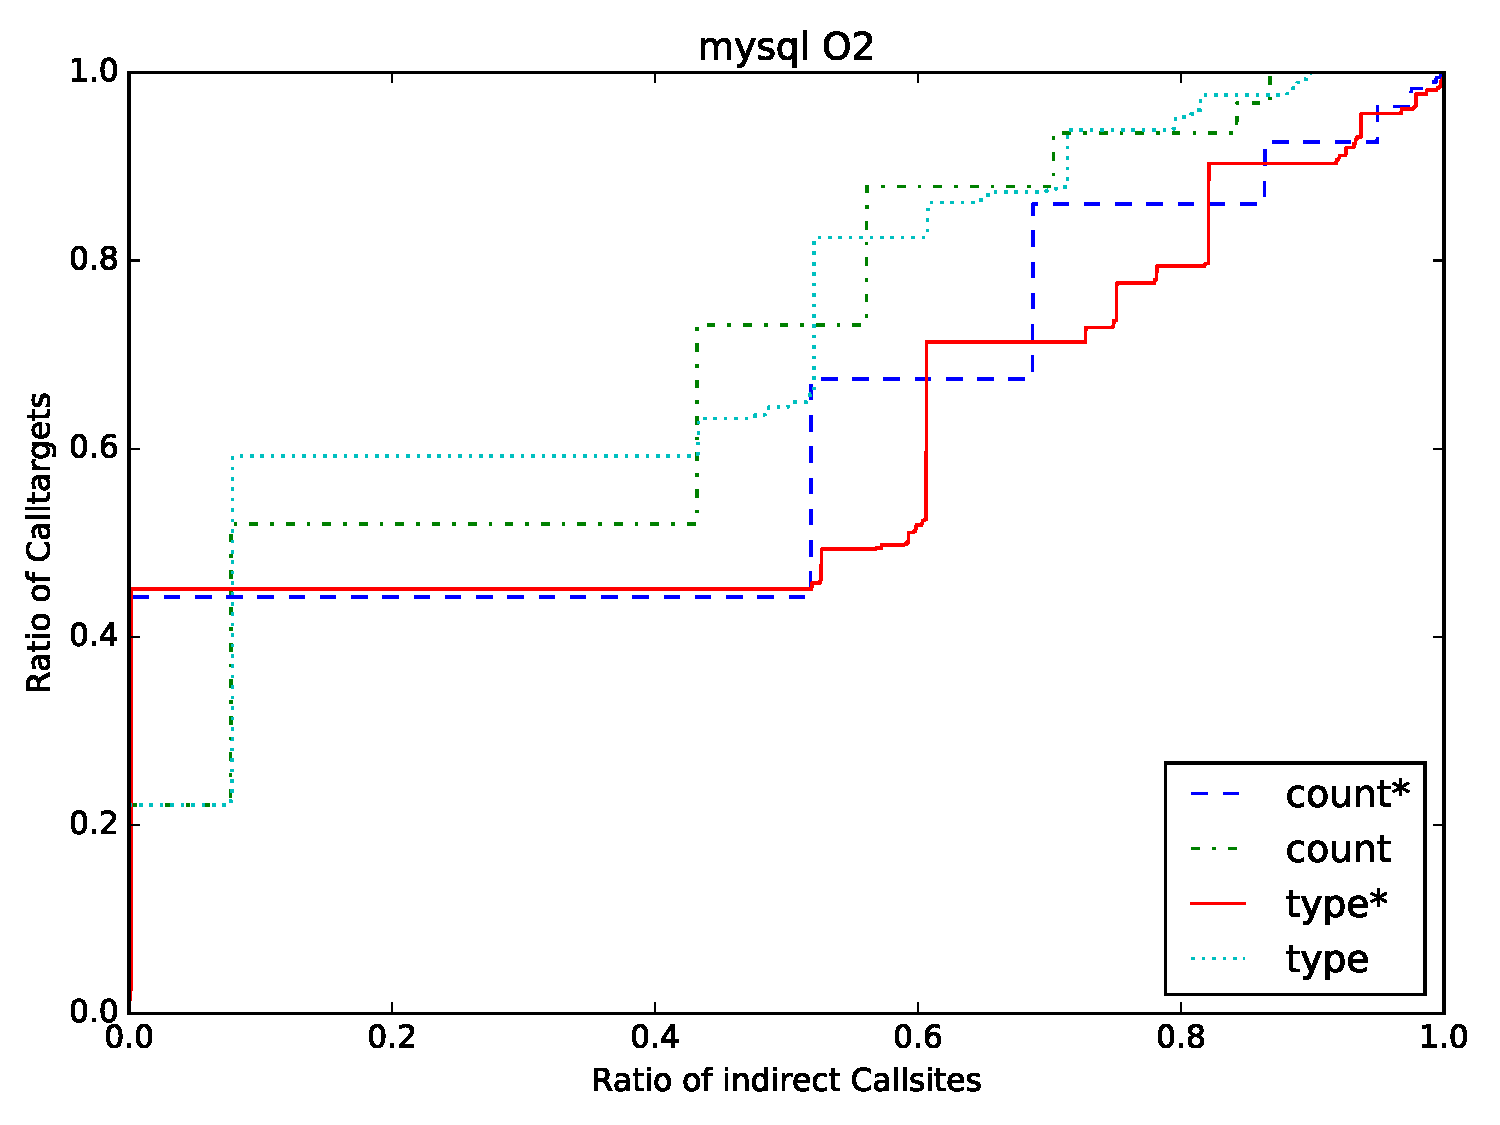
\includegraphics[width=0.5\textwidth]{../MA_Pictures/mysql.pdf}\\
%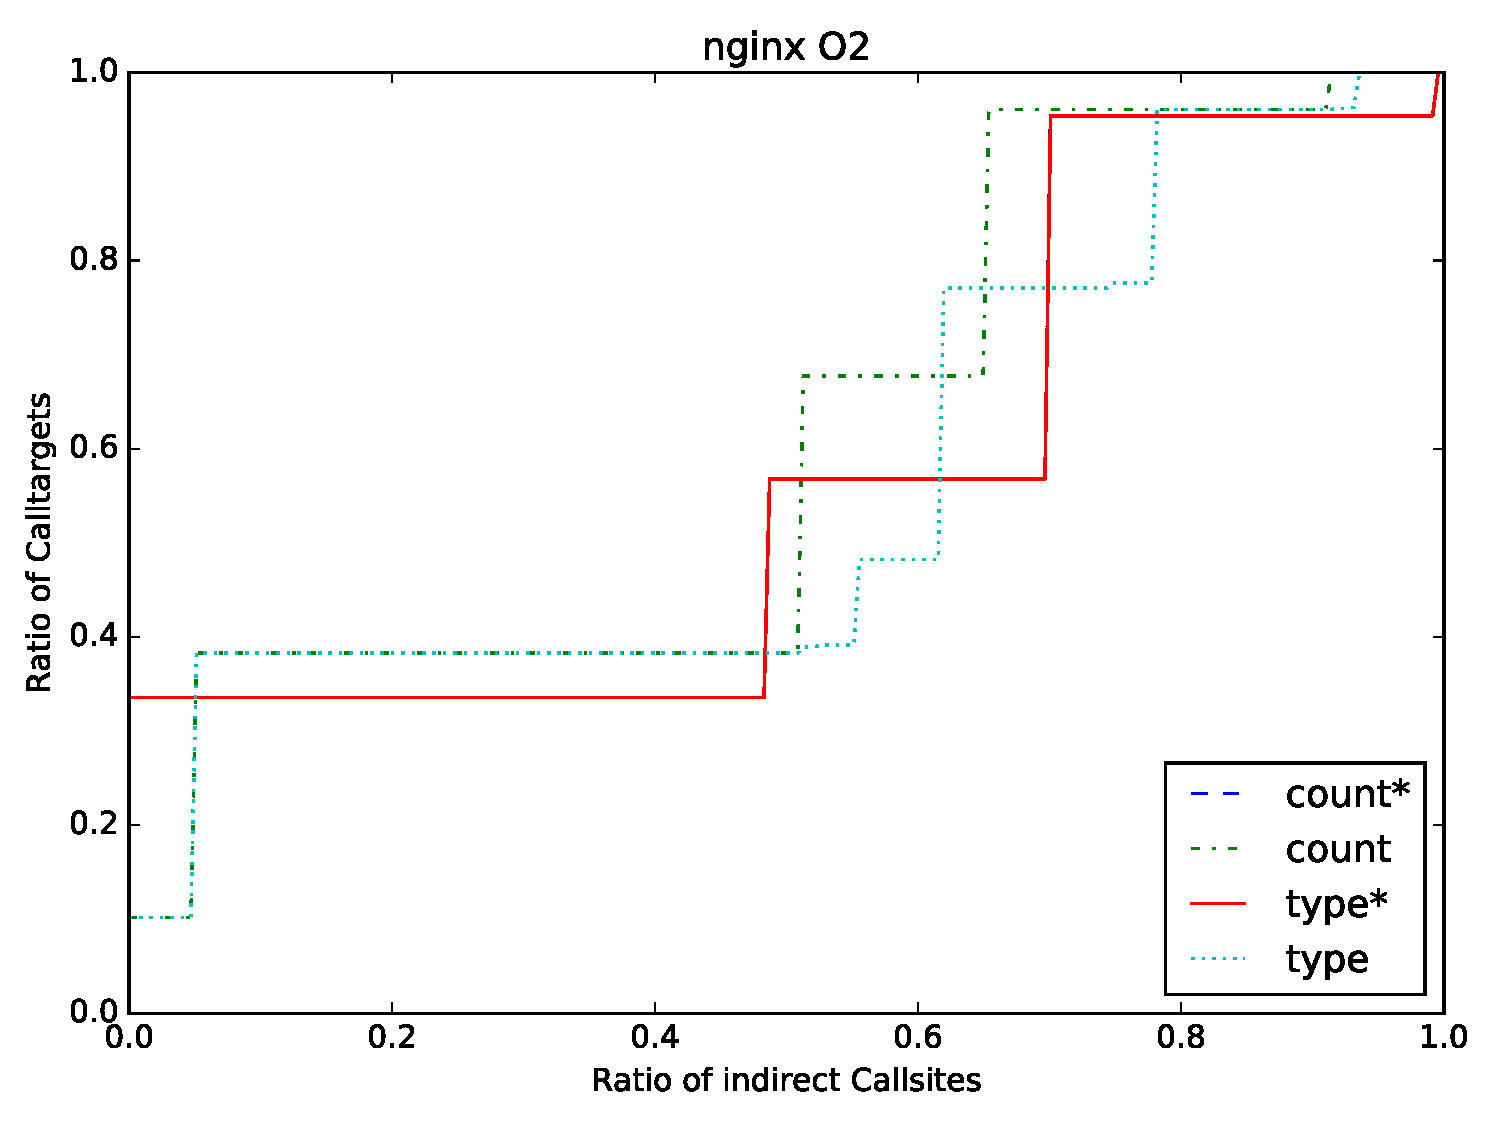
\includegraphics[width=0.5\textwidth]{../MA_Pictures/nginx.pdf}
%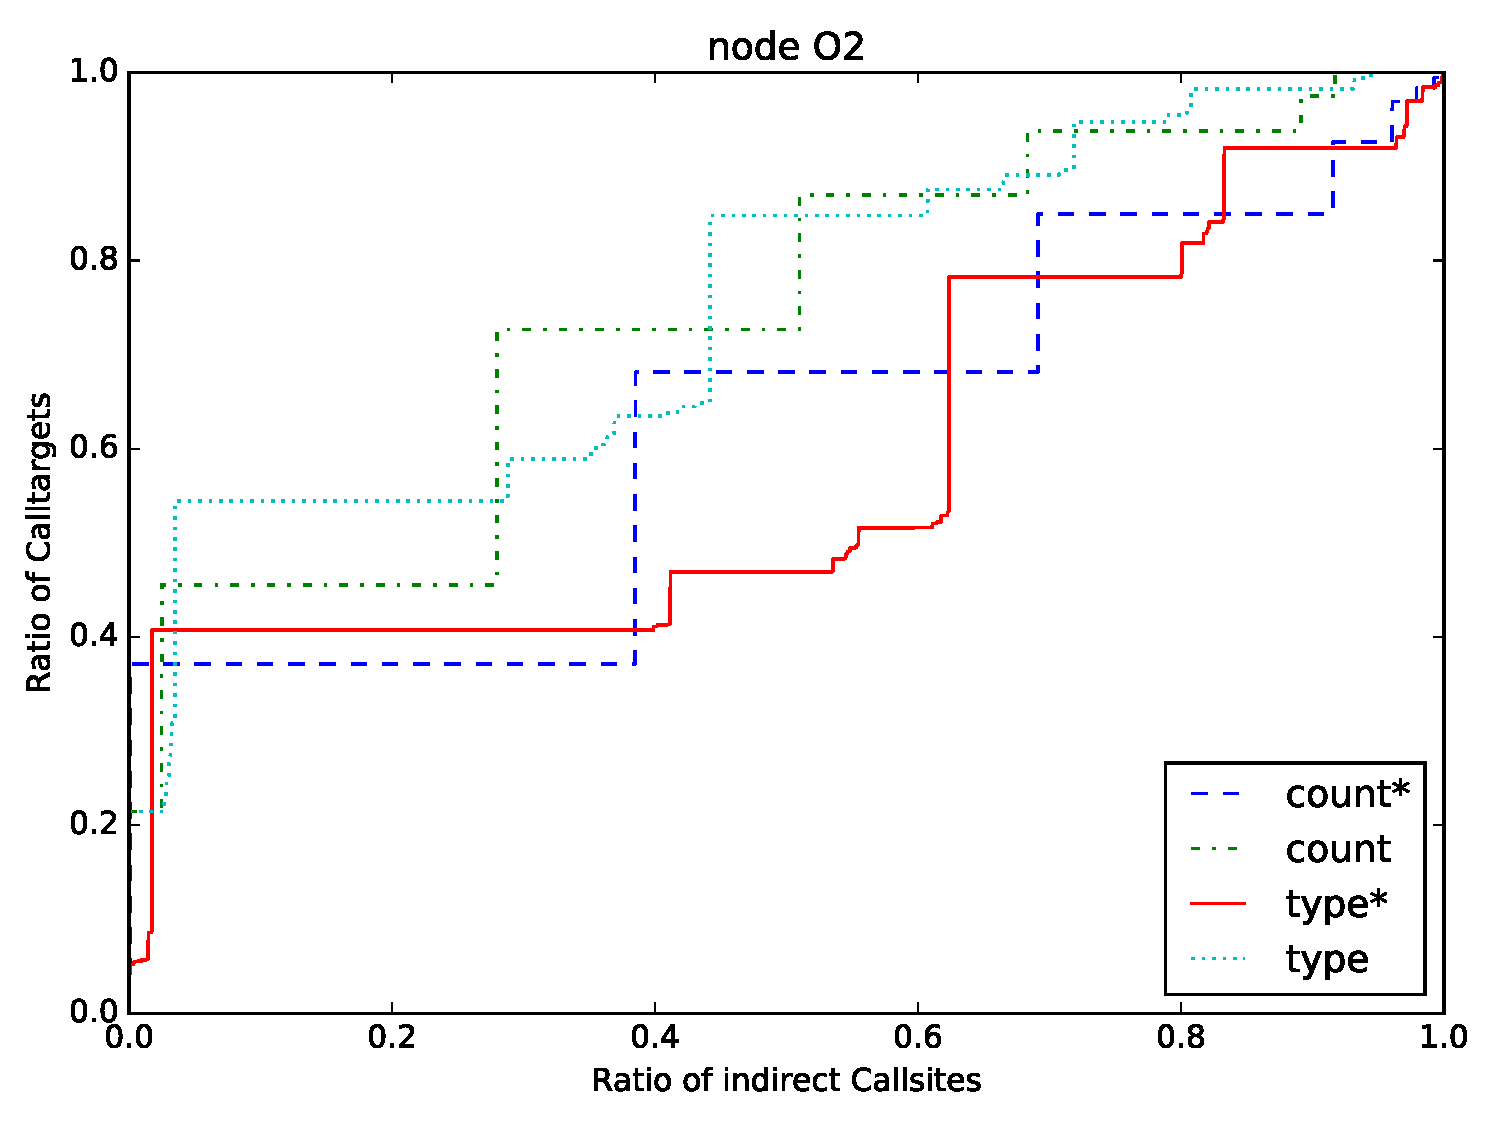
\includegraphics[width=0.5\textwidth]{../MA_Pictures/node.pdf}\\
%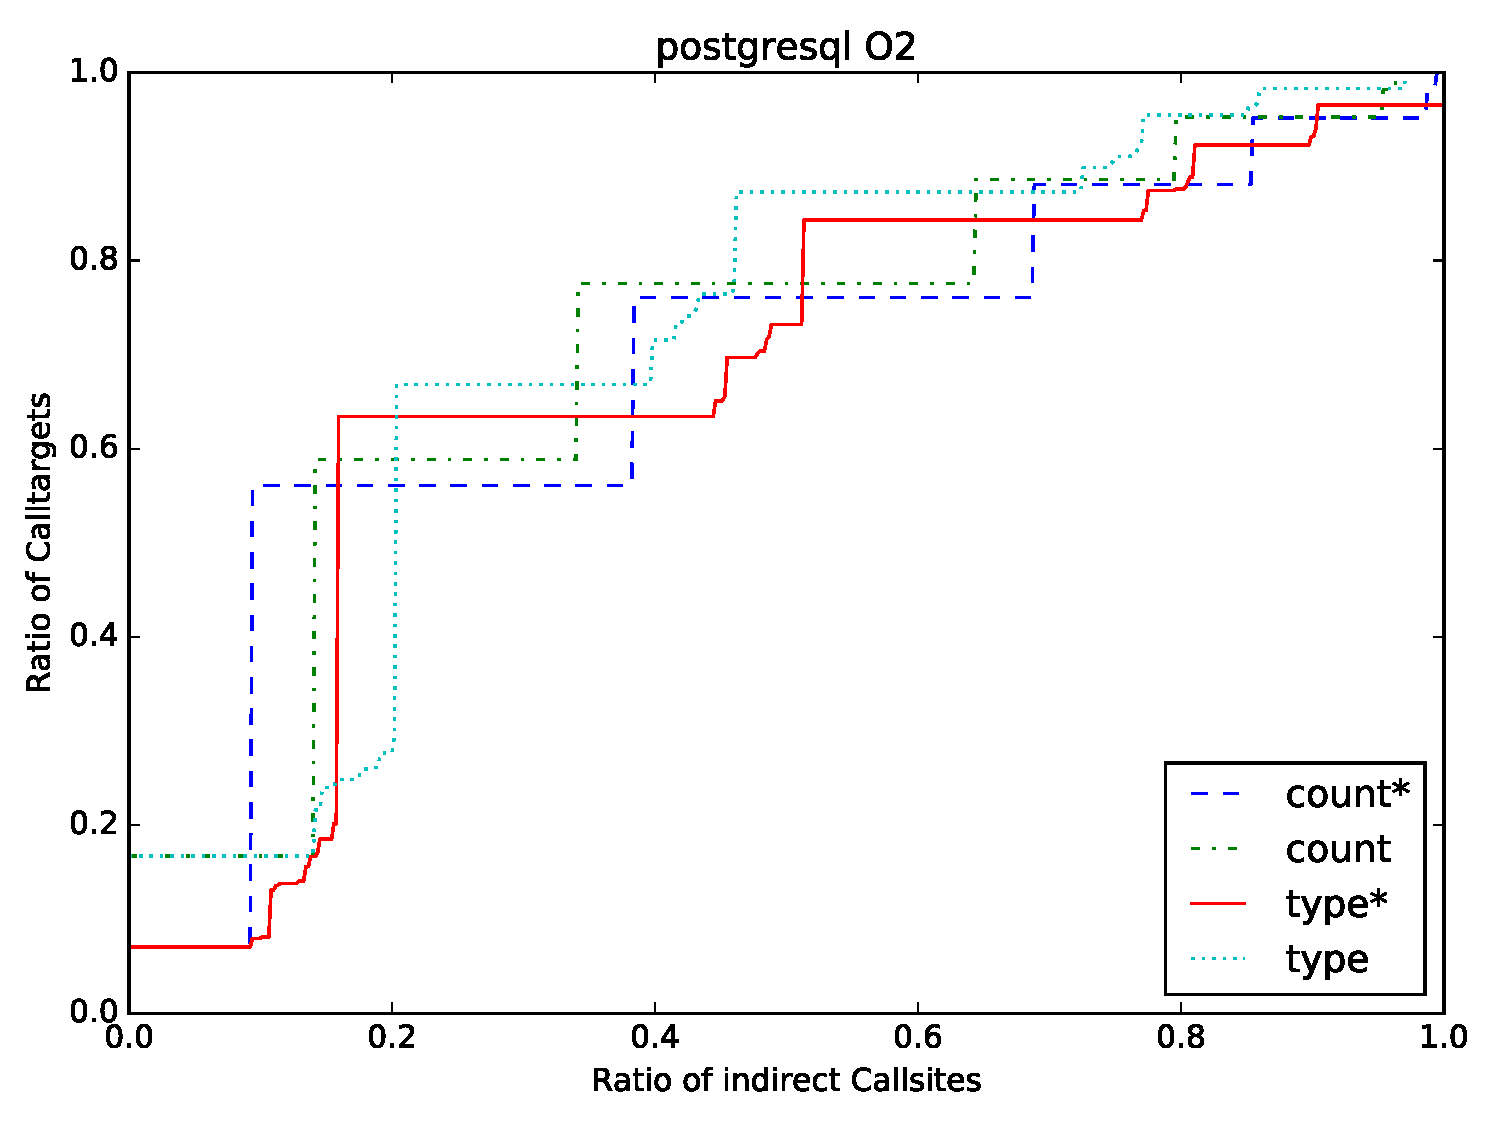
\includegraphics[width=0.5\textwidth]{../MA_Pictures/postgresql.pdf}
%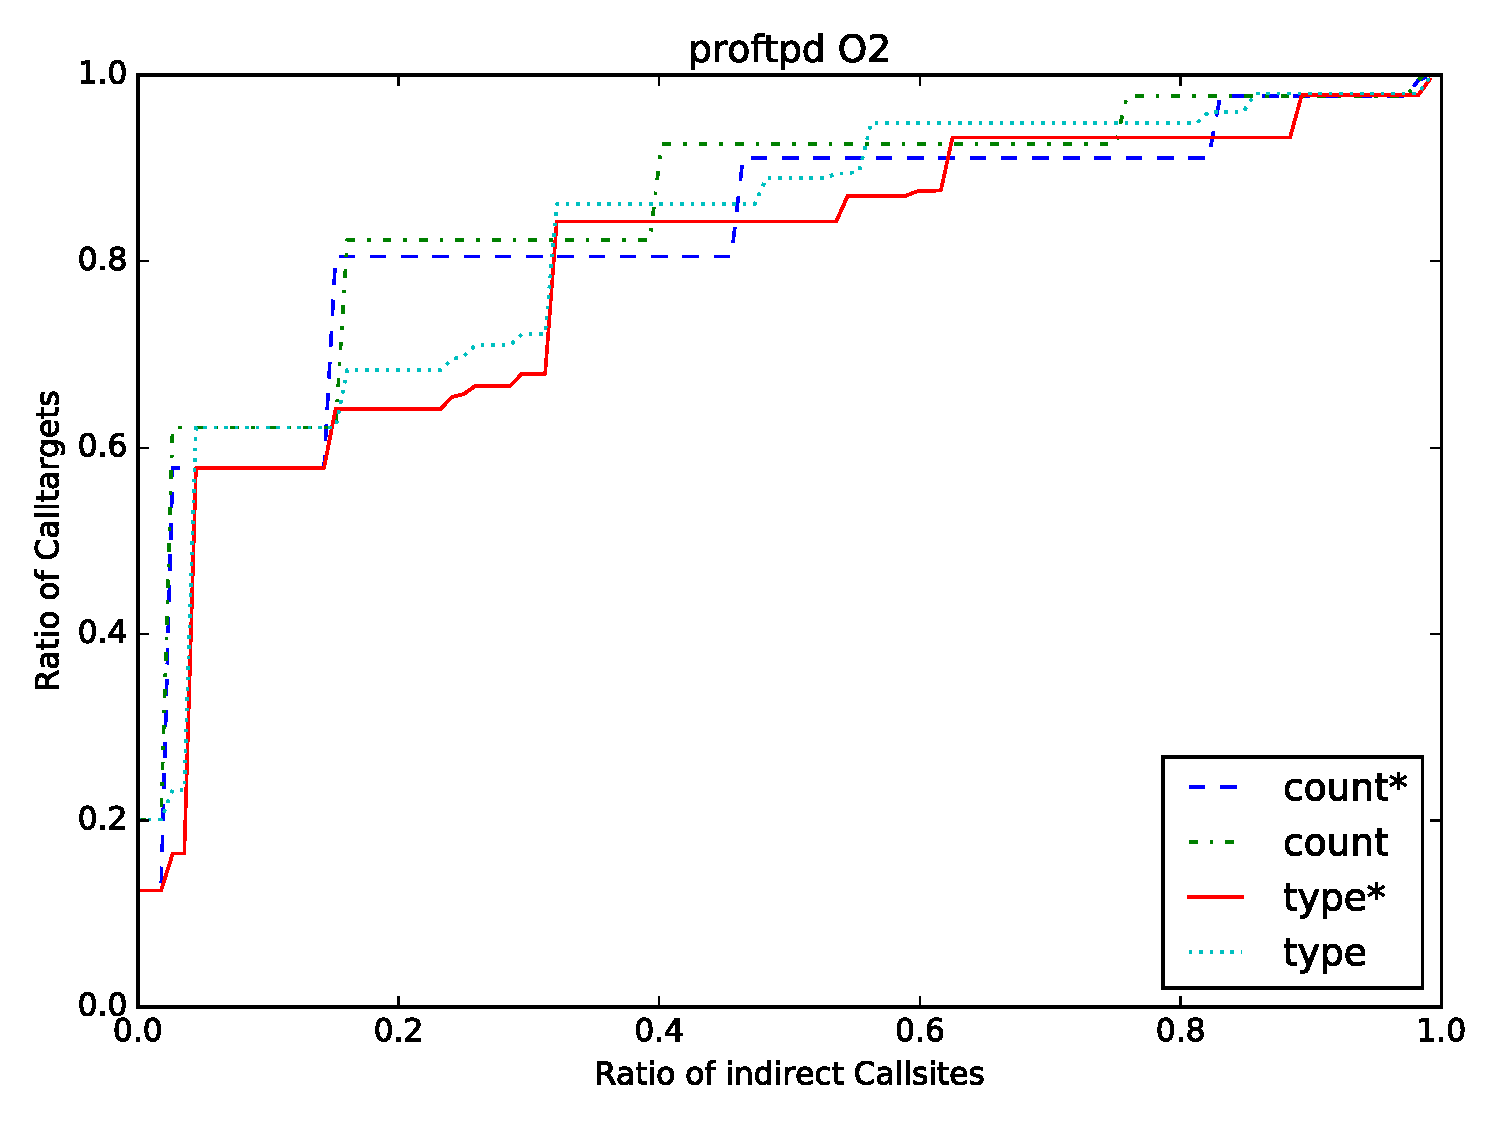
\includegraphics[width=0.5\textwidth]{../MA_Pictures/proftpd.pdf}
%\end{figure}
%


%
%\subsection{RQ3: Runtime Performance Overhead}
%\label{section:typeshieldoverheadperformance}
%\todo[inline]{In this section we need one or two Table similar to what TypeArmor contains, first we need to define the fields which make most sense.}
%Here we measure how much performance overhead the instrumentation incurs.
%Here we measure with the same SPEC2006 programs that was used in the TypeArmor paper.
%spec 2006.
%\todo[inline]{add a binary patch that does not crash none of the programs from SPEC2006.}
%\todo[inline]{need a table with all the results for each of the SPEC2006 programs and a bar diagram}
%
%\subsection{RQ4: Instrumentation Overhead}
%\label{section:typeshieldoverheadinstrumentation}
%\todo[inline]{here we need a bar chart, see TypeArmor paper.}
%Here we measure how much the binaries increased in size after the instrumentation was added to the binaries.
%\todo[inline]{Measure the size (in bytes) of the SPEC2006 testes in RQ3 before and after adding all the patches}
%



% \subsection{RQ5: Security Level of \textsc{TypeShield}}
% \label{section:mitiagtion}
% \todo[inline]{here we need a a CDF figure, see the TypeAmor paper w.r.t. security analysis in the evaluation. The buckets have to be defined first, reason about if they make sense!}
% We look at our implementation conceptually and assess qualitatievly whether our implementation can interfere with various classes of attacks. 
% \todo[inline]{see the TypeAmor paper w.r.t. security analysis in the evaluation, a CDF figure is here required.}
% 
% \subsection{RQ6: Add another evaluation dimention we did not think off, maybe ``RQ6: TypeShield Deployments" (if it is easy or hard to deploy our tool in
% comparison with TypeArmor.)}
% \label{section:mitiagtion}
% \todo[inline]{need to define first the question.}




% \begin{figure}
% \centering
% \def\svgwidth{columnwidth}
% \input{postgresqlO2.pdf_tex}
% \end{figure}

% \subsection{COOP}
% \label{Effectiveness against COOP}
% 
% \subsubsection{COOP Extensions}
% \label{COOP Extensions}
% 
% \subsubsection{Pure Data-only Attacks}
% \label{Pure Data-only Attacks}
